% Generated by code/ch13_twoqubit_id.py -- do not edit by hand.
\definecolor{qocA}{rgb}{0.00,0.45,0.70}
\definecolor{qocB}{rgb}{0.90,0.60,0.00}
\definecolor{qocC}{rgb}{0.00,0.62,0.45}
\definecolor{qocD}{rgb}{0.80,0.40,0.00}
\definecolor{qocE}{rgb}{0.80,0.60,0.70}
\definecolor{qocF}{rgb}{0.35,0.70,0.90}
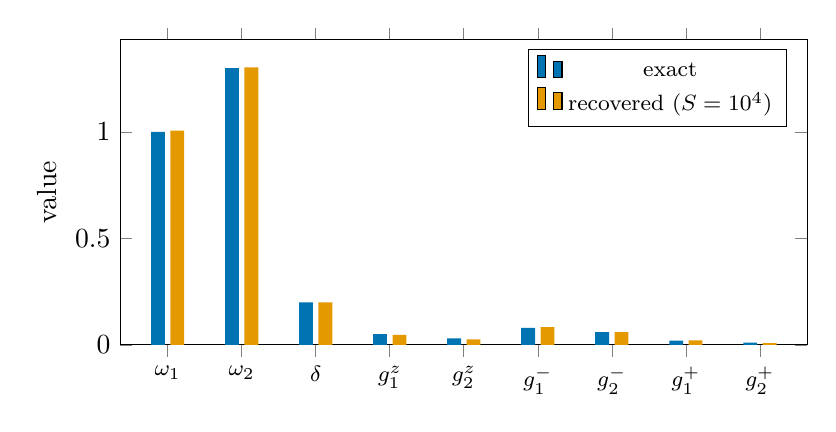
\begin{tikzpicture}[]
\begin{axis}[ybar, bar width=5pt, width=0.85\linewidth, height=0.45\linewidth, ylabel={value},
  symbolic x coords={$\omega_1$,$\omega_2$,$\delta$,$g^z_1$,$g^z_2$,$g^-_1$,$g^-_2$,$g^+_1$,$g^+_2$}, xtick=data, x tick label style={font=\footnotesize},
  legend style={font=\footnotesize}, legend pos=north east, ymin=0, enlarge x limits=0.08]
\addplot[fill=qocA, draw=none] coordinates {($\omega_1$,1.0000) ($\omega_2$,1.3000) ($\delta$,0.2000) ($g^z_1$,0.0500) ($g^z_2$,0.0300) ($g^-_1$,0.0800) ($g^-_2$,0.0600) ($g^+_1$,0.0200) ($g^+_2$,0.0100)};
\addplot[fill=qocB, draw=none] coordinates {($\omega_1$,1.0061) ($\omega_2$,1.3026) ($\delta$,0.1999) ($g^z_1$,0.0473) ($g^z_2$,0.0260) ($g^-_1$,0.0828) ($g^-_2$,0.0597) ($g^+_1$,0.0210) ($g^+_2$,0.0078)};
\legend{exact, recovered ($S=10^4$)}
\end{axis}
\end{tikzpicture}
